\documentclass[tikz,border=20pt]{standalone}
\usepackage{pgfplots}
\pgfplotsset{compat=1.18} % Ensure compatibility with modern pgfplots features

\begin{document}
	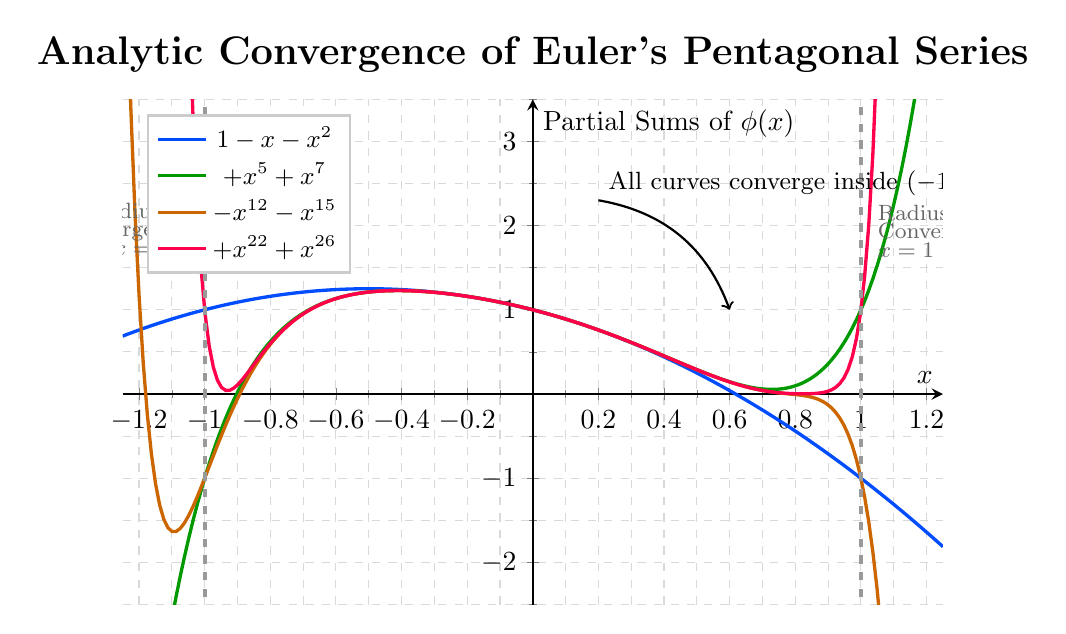
\begin{tikzpicture}
		\begin{axis}[
			width=12cm, height=8cm,
			title={\Large \textbf{Analytic Convergence of Euler's Pentagonal Series}},
			xlabel={$x$},
			ylabel={Partial Sums of $\phi(x)$},
			xmin=-1.25, xmax=1.25,
			ymin=-2.5, ymax=3.5,
			axis lines=middle,
			samples=200, % High sample rate for smooth curves
			domain=-1.25:1.25,
			legend pos=north west,
			legend style={draw=black!20, fill=white!90, font=\small},
			thick,
			grid=both,
			grid style={dashed, gray!30},
			minor tick num=1
			]
			
			% ==========================================
			% PARTIAL SUM POLYNOMIALS
			% ==========================================
			
			% S_2: 1 - x - x^2
			\addplot [color=blue!70!cyan, very thick] {1 - x - x^2};
			\addlegendentry{$1 - x - x^2$}
			
			% S_7: 1 - x - x^2 + x^5 + x^7
			\addplot [color=green!60!black, very thick] {1 - x - x^2 + x^5 + x^7};
			\addlegendentry{$+ x^5 + x^7$}
			
			% S_15: 1 - x - x^2 + x^5 + x^7 - x^12 - x^15
			\addplot [color=orange!80!black, very thick] {1 - x - x^2 + x^5 + x^7 - x^12 - x^15};
			\addlegendentry{$- x^{12} - x^{15}$}
			
			% S_26: 1 - x - x^2 + x^5 + x^7 - x^12 - x^15 + x^22 + x^26
			\addplot [color=red!70!magenta, very thick] {1 - x - x^2 + x^5 + x^7 - x^12 - x^15 + x^22 + x^26};
			\addlegendentry{$+ x^{22} + x^{26}$}
			
			% ==========================================
			% RADIUS OF CONVERGENCE BOUNDARIES
			% ==========================================
			% Draw asymptotes at x = -1 and x = 1
			\draw[dashed, gray!80, line width=1.5pt] (axis cs:-1,-3) -- (axis cs:-1,4);
			\draw[dashed, gray!80, line width=1.5pt] (axis cs:1,-3) -- (axis cs:1,4);
			
			% Annotations for the boundaries
			\node[anchor=south west, text=gray!80!black, font=\footnotesize, align=left] 
			at (axis cs:1.02, 1.5) {Radius of\\[-1mm]Convergence\\[-1mm]$x = 1$};
			
			\node[anchor=south east, text=gray!80!black, font=\footnotesize, align=right] 
			at (axis cs:-1.02, 1.5) {Radius of\\[-1mm]Convergence\\[-1mm]$x = -1$};
			
			% Annotate behavior near x=1
			\node[anchor=west, text=black, font=\small] at (axis cs:0.2, 2.5) {All curves converge inside $(-1, 1)$};
			\draw[->, thick] (axis cs:0.2, 2.3) to[bend left] (axis cs:0.6, 1);
			
		\end{axis}
	\end{tikzpicture}
\end{document}